\chapter[一个模型系统的态]{一个模型系统的态\footnote{原文:model system ——译者注}}

热力学物理是统计和力学原理联合的结果。力学告诉我们功的释义,热力学告诉我们热的释义。热力学物理中会出现普通力学中没有的三个量:熵、温度和自由能。我们将在前三个章节介绍它们的定义,在此之后推算出一些关于此的结果。

我们研究热物理学的出发点是粒子系统的静止量子态的概念。当我们计算一个系统的可能量子态时,根据熵定义为态数的自然对数(第二章),我们可以知道系统的熵。熵对系统温度的依赖定义了温度。从熵、温度和自由能中,我们可以找到系统的压力、化学势和所有其他的热力学性质。

对于一个处于静止量子态的系统,所有可观测的物理性质,如能量和粒子的数量,都与时间无关。为了简洁起见,我们通常省略静止这个词;我们所处理的量子态是静止的,除非我们在第14-15章中讨论输运过程。我们所讨论的系统可以由单个粒子组成,或者更常见地是由许多粒子组成。该理论是为了处理相互作用粒子的封闭系统而发展起来的,但在相互作用可能被忽略的特定问题上,可以强有力地简化。

每个量子态都有一个确定的能量。稳定的。。。

\begin{figure}[ht]
    \centering % centering figure
    \scalebox{0.8} % rescale the figure by a factor of 0.8
    {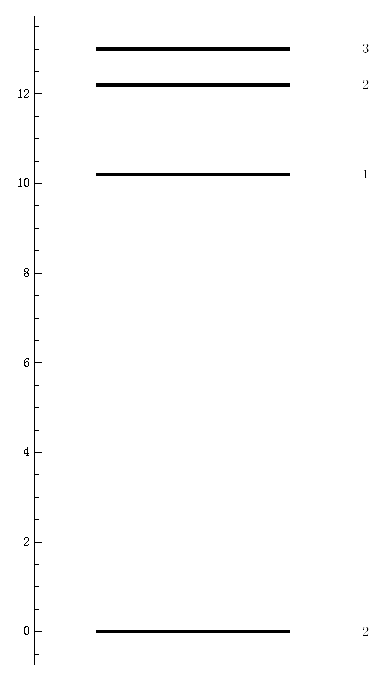
\includegraphics{chapters/ch1/11.eps}} % importing figure
    \label{fig:11} % labeling to refer it inside the text
   \end{figure}

\section{二元模型系统}